\documentclass{article}
\usepackage{geometry}
\usepackage{titling}
\usepackage{hyperref}
\usepackage{amsmath}
\usepackage{amssymb}
\usepackage{graphicx}
\usepackage{caption}
\usepackage{subcaption}
\usepackage{stmaryrd}
\usepackage[dvipsnames]{xcolor}

\geometry{
  a4paper,
  total = {170mm, 257mm},
  left = 20mm,
  top = 20mm,
}
\graphicspath{ {./images/} }

\newcommand{\addfig}[2]{\begin{figure}[!htb] \centering \includegraphics[width=#1\textwidth]{#2}\end{figure}}

\newcommand{\aexp}[1]{\langle\text{#1}\rangle}
\newcommand{\intexp}{\aexp{intexp}}
\newcommand{\var}{\aexp{var}}
\newcommand{\assert}{\aexp{assert}}
\newcommand{\sem}[1]{\left\llbracket #1\right\rrbracket}

\newcommand{\N}{\mathbb{N}}
\newcommand{\Z}{\mathbb{Z}}


\title{Trabajo práctico N° 2}
\author{Emanuel Nicolás Herrador}
\date{Abril 2025}

\makeatletter
\def\@maketitle{%
  \newpage
  \null
  \vskip 1em%
  \begin{center}%
  \let \footnote \thanks
    {\LARGE \@title \par}%
    \vskip 1em%
    {\large \@date}%
  \end{center}%
  \par
  \vskip 1em}
\makeatother

\begin{document}

\maketitle

\noindent\begin{tabular}{@{}ll}
	Estudiante & \theauthor \\
\end{tabular}

\section*{Repaso}
Veamos cada punto por separado:
\begin{enumerate}
	\item Si $\sem{-}$ no es inyectiva, entonces no es una función semántica: \textbf{Falso} porque diferentes expresiones pueden tener la misma semántica.
	      Por ejemplo, para la semántica de expresiones enteras, $\sem{1+2} = \sem{2+1}$.
	\item Si $\sem{-}$ no es suryectiva, entonces no es una función semántica: \textbf{Falso} porque para ser función semántica solo se requiere que cada frase abstracta tenga un solo significado semántico.
	      Es decir, no se requiere que se abarquen todos los elementos del dominio semántico como significados de las frases abstractas, sino solo que la función sea total.
	\item La dirección por sintaxis garantiza que un conjunto de ecuaciones define una función semántica: \textbf{Verdadero} porque en particular la dirección de sintaxis garantiza que cada frase abstracta está representada por una sola ecuación semántica.
	      Además, garantiza que cada ecuación semántica tiene un significado en función de la semántica de sus subfrases inmediatas, lo cual garantiza que la recursividad en la definición tiene un fin y una definición única.
	      Por ello, esto garantiza que la función resultante es total y, por ende, una función semántica.
	\item Si un conjunto de ecuaciones que define una semántica no es dirigido por sintaxis, entonces la semántica no es composicional: \textbf{Falso} por contraejemplo dado que la función de la semántica de números binarios del ejercicio $5$ de la guía anterior era una función semántica no dirigida por sintaxis.
\end{enumerate}

\section*{Ejercicio 1}
Notemos que las dos expresiones que tenemos son equivalentes dado que una es la división entera y la otra su definición:
\begin{equation*}
	\begin{aligned}
		x \div y                  & = z                   \\
		\exists r. (0 \leq r < y) & \land (x = y * z + r)
	\end{aligned}
\end{equation*}

Sin embargo, dado que en nuestra semántica la división por cero sí tiene un significado, i.e. está definido, es claro notar que sea $n \in \Z$ el valor para el cual se cumple $\forall e \in \intexp : (\sem{e \div 0} = n)$, la primera expresión puede considerarlo mientras que la segunda no.
Es decir, un estado que genera distinta semántica puede ser $\sigma = \{(x, 1), (y, 0), (z, n), \dots\}$.
De este modo, otorgando lo valores del estado, tenemos que:
\begin{equation*}
	\begin{aligned}
		\sem{x \div y = z} \sigma                                    & = \sem{1 \div 0 = n} = 1                                    \\
		\sem{\exists r. (0 \leq r < y) \land (x = y * z + r)} \sigma & = \sem{\exists r. (0 \leq r < 0) \land (1 = 0 * n + r)} = 0
	\end{aligned}
\end{equation*}

Por lo que son distintas semánticas las que se obtienen.

Respecto a la caracterización de los estados para los cuales los predicados tienen la misma semántica, son todos aquellos donde la división entera es correcta y está definida.
Es decir, $\sigma_2 = \{(x, n_1), (y, n_2), (z, n_1 \div n_2), \dots\}$ para $n_1 \in \Z$ y $n_2 \in \Z - \{0\}$.

\section*{Ejercicio 2}
Para extender la gramática de las expresiones enteras para agregar la sumatoria, vamos a considerar algo de la forma:
\begin{equation*}
	\sum_{\var = \intexp}^{\intexp} \intexp
\end{equation*}
de modo que la definición sea:
\begin{equation*}
	\sem{\sum_{i = e_0}^{e_1} e} \sigma = \sum_{n_i = \sem{e_0} \sigma}^{\sem{e_1} \sigma} \sem{e} [\sigma | i : n_i]
\end{equation*}

\section*{Ejercicio 3}
Consideraremos que las ocurrencias ligadoras son las subrayadas, las ligadas las envueltas en un círculo y las libres las envueltas en un cuadrado.
Las ocurrencias ligadas están ligadas a la ocurrencia ligadora del mismo color.

\begin{figure}[!htb]
	\centering
	\begin{subfigure}[b]{0.4\textwidth}
		\centering
		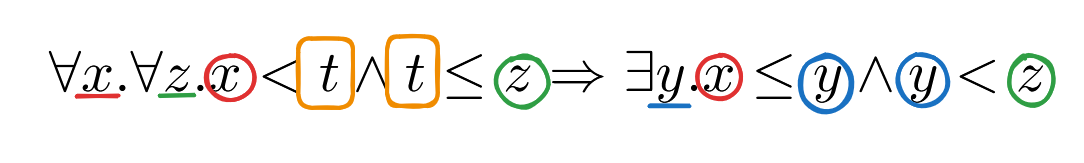
\includegraphics[width=\textwidth]{02-03-a.png}
	\end{subfigure}
	\hfil
	\begin{subfigure}[b]{0.4\textwidth}
		\centering
		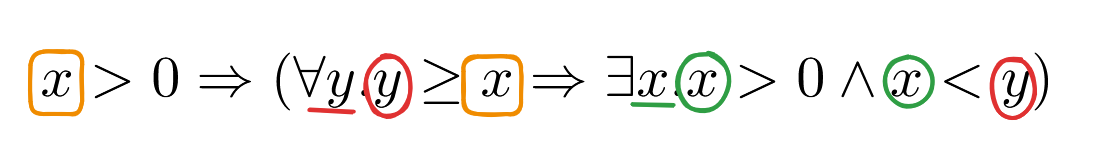
\includegraphics[width=\textwidth]{02-03-b.png}
	\end{subfigure}
	\hfil
	\begin{subfigure}[b]{0.25\textwidth}
		\centering
		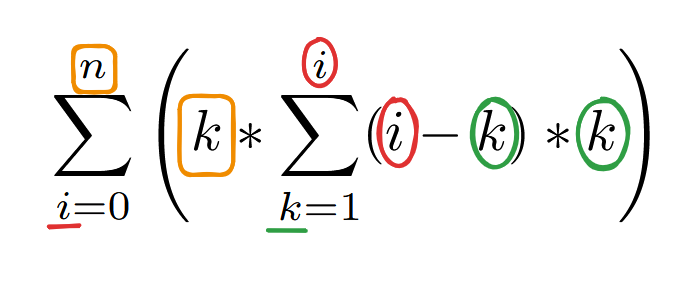
\includegraphics[width=\textwidth]{02-03-c.png}
	\end{subfigure}
\end{figure}

\section*{Ejercicio 4}

\subsection*{Item A}
Veamos primero las variables libres para cada frase abstracta que conforma la expresión:
\begin{equation*}
	\begin{aligned}
		FV(\forall x. \forall z. x < t \land t \leq z \Rightarrow \exists y. x \leq y \land y < z) & = FV(\forall z. x < t \land t \leq z \Rightarrow \exists y. x \leq y \land y < z) - \{x\} \\
		                                                                                           & = \{y, t\}                                                                                \\
		FV(\forall z. x < t \land t \leq z \Rightarrow \exists y. x \leq y \land y < z)            & = FV(x < t \land t \leq z \Rightarrow \exists y. x \leq y \land y < z) - \{z\}            \\
		                                                                                           & = \{x, y, t\}                                                                             \\
		FV(x < t \land t \leq z \Rightarrow \exists y. x \leq y \land y < z)                       & = FV(x < t \land t \leq z) \cup FV(\exists y. x \leq y \land y < z)                       \\
		                                                                                           & = \{x, y, z, t\}                                                                          \\
		FV(x < t \land t \leq z)                                                                   & = FV(x < y) \cup FV(t \leq z)                                                             \\
		                                                                                           & = FV(x) \cup FV(y) \cup FV(t) \cup FV(z)                                                  \\
		                                                                                           & = \{x, y, z, t\}                                                                          \\
		FV(\exists y. x \leq y \land y < z)                                                        & = FV(x \leq y \land y < z) - \{y\}                                                        \\
		                                                                                           & = \{x, z\}                                                                                \\
		FV(x \leq y \land y < z)                                                                   & = FV(x \leq y) \cup FV(y < z)                                                             \\
		                                                                                           & = FV(x) \cup FV(y) \cup FV(y) \cup FV(z)                                                  \\
		                                                                                           & = \{x, y, z\}
	\end{aligned}
\end{equation*}

Con ello, si consideramos la sustitución $\delta : \var \to \intexp$ tal que $\delta t = x + y + z$ y $\delta w = w\ \forall w \neq t$, entonces el reemplazo simultáneo nos queda:
\begin{equation*}
	\begin{aligned}
		 & \qquad (\forall x. \forall z. x < t \land t \leq z \Rightarrow \exists y. x \leq y \land y < z)/\delta =                                                  \\
		 & = \forall x_{new}. (\forall z. x < t \land t \leq z \Rightarrow \exists y. x \leq y \land y < z)/[\delta | x : x_{new}]                                   \\
		 & \qquad \text{tal que } x_{new} \notin \bigcup_{w \in FV(\forall x \dots)} FV(\delta w) = FV(\delta y) \cup FV(\delta t)                                   \\
		 & \qquad \text{i.e., } x_{new} \notin \{x, y, z\}                                                                                                           \\
		 & = \forall k. (\forall z. x < t \land t \leq z \Rightarrow \exists y. x \leq y \land y < z)/[\delta | x : k]                                               \\
		 & = \forall k. \forall z_{new}. (x < t \land t \leq z \Rightarrow \exists y. x \leq y \land y < z)/[\delta | x : k | z : z_{new}]                           \\
		 & \qquad \text{tal que } z_{new} \notin \bigcup_{w \in FV(\forall z \dots)} FV([\delta | x : k] w) = \{k, y, z, x\}                                         \\
		 & = \forall k. \forall s. (x < t \land t \leq z \Rightarrow \exists y. x \leq y \land y < z)/[\delta | x : k | z : s]                                       \\
		 & = \forall k. \forall s. (x < t \land t \leq z)/[\delta | x : k | z : s] \Rightarrow (\exists y. x \leq y \land y < z)/[\delta | x : k | z : s]            \\
		 & = \forall k. \forall s. (k < x + y + z \land x + y + z \leq s) \Rightarrow \exists y_{new}. (x \leq y \land y < z)/[\delta | x : k | z : s | y : y_{new}] \\
		 & \qquad \text{tal que } y_{new} \notin \bigcup_{w \in FV(\exists y \dots)} FV([\delta | x : k | z : s] w) = \{k, s\}                                       \\
		 & = \forall k. \forall s. (k < x + y + z \land x + y + z \leq s) \Rightarrow \exists y. (x \leq y \land y < z)/[\delta | x : k | z : s]                     \\
		 & = \forall k. \forall s. (k < x + y + z \land x + y + z \leq s) \Rightarrow \exists y. (k \leq y \land y < s)
	\end{aligned}
\end{equation*}

\subsection*{Item B}
Vamos a hacer un razonamiento análogo al del ejercicio anterior pero sin expandir tan a detalle el cálculo de las variables libres dado que es algo sencillo de ver.
Por ello, la sustitución $\delta$ a considerar es:
\begin{equation*}
	\delta w = \begin{cases}
		x & \text{si } w = y \\
		y & \text{si } w = z \\
		z & \text{si } w = x \\
		w & \text{cc.}
	\end{cases}
\end{equation*}

Con esto en mente, tenemos:
\begin{equation*}
	\begin{aligned}
		 & \qquad (x > 0 \Rightarrow (\forall y. y \geq x \Rightarrow \exists x. x > 0 \land x < y))/\delta =                            \\
		 & = (x > 0)/\delta \Rightarrow (\forall y. y \geq x \Rightarrow \exists x. x > 0 \land x < y)/\delta                            \\
		 & = (z > 0) \Rightarrow \forall y. (y \geq x \Rightarrow \exists x. x > 0 \land x < y)/[\delta | y : y_{new}]                   \\
		 & \qquad \text{tal que } y_{new} \notin \bigcup_{w \in FV(\forall y \dots)} FV(\delta w) = \{z\}                                \\
		 & = (z > 0) \Rightarrow \forall y. (y \geq x \Rightarrow \exists x. x > 0 \land x < y)/[\delta | y : y])                        \\
		 & = (z > 0) \Rightarrow (\forall y. (y \geq x)/[\delta | y : y] \Rightarrow (\exists x. x > 0 \land x < y)/[\delta | y : y])    \\
		 & = (z > 0) \Rightarrow (\forall y. (y \geq z) \Rightarrow \exists x_{new}. (x > 0 \land x < y)/[\delta | y : y | x : x_{new}]) \\
		 & \qquad \text{tal que } x_{new} \notin \bigcup_{w \in FV(\exists x \dots)} FV([\delta | y : y] w) = \{y\}                      \\
		 & = (z > 0) \Rightarrow (\forall y. (y \geq z) \Rightarrow \exists x. (x > 0 \land x < y)/[\delta | y : y | x : x])             \\
		 & = (z > 0) \Rightarrow (\forall y. (y \geq z) \Rightarrow \exists x. (x > 0 \land x < y))
	\end{aligned}
\end{equation*}

\section*{Ejercicio 5}
El ejemplo que muestra que hacer reemplazo sintáctico en lugar de sustitución es cuando consideramos $\delta y = x$ para $(\exists x. x > y)$.
Esto sucede dado que $\sem{(\exists x. x > x)} = 0$ mientras que $\sem{(\exists x. x > y)} = 1$.

\section*{Ejercicio 6}
Queremos ver, por inducción en los predicados $p$ que $FV(p/\delta) = \bigcup_{w \in FV(p)} FV(\delta w)$.
Para ello, veamos cada parte de nuestra inducción:
\begin{itemize}
	\item \textbf{Caso base}: Tenemos dos tipos de casos base, los de $\text{true}$ y $\text{false}$, y los que involucran expresiones enteras.
	      Observando el primer tipo, dado que es análogo para ambos solo vamos a detallar uno.
	      Por esto, tenemos:
	      \begin{equation*}
		      \begin{aligned}
			      FV(\text{true}/\delta) = FV(\text{true})                                              & = \emptyset \\
			      \bigcup_{w \in FV(\text{true})} FV(\delta w) = \bigcup_{w \in \emptyset} FV(\delta w) & = \emptyset
		      \end{aligned}
	      \end{equation*}
	      Por lo que se demuestra para este tipo de caso base.

	      Ahora, respecto a los que involucran expresiones, al tener siempre operadores binarios, vamos a extenderlo para $\varolessthan \in \{<, >, \leq, \geq, =, \neq\}$:
	      \begin{equation*}
		      \begin{aligned}
			      FV((e \varolessthan e')/\delta) = FV(e/\delta \varolessthan e'/\delta)                               & = FV(e/\delta) \cup FV(e'/\delta)                                                                       \\
			      \bigcup_{w \in FV(e \varolessthan e')} FV(\delta w) = \bigcup_{w \in FV(e) \cup FV(e')} FV(\delta w) & = \left(\bigcup_{w \in FV(e)} FV(\delta w)\right) \cup \left(\bigcup_{w \in FV(e')} FV(\delta w)\right)
		      \end{aligned}
	      \end{equation*}
	      Finalmente, notemos que al ser expresiones enteras, todas sus variables son libres.
	      Luego, es trivial ver que es correcto decir $FV(e/\delta) = \bigcup_{w \in FV(e)} FV(\delta w)\ \forall e \in \intexp$ dado que la sustitución se realiza para todas las variables de $e$ sin excepción.
	      Por ello, entonces, se demuestra este segundo tipo de caso de base.

	      Viendo todo lo anterior, se demuestra todo el caso base. $\blacksquare$

	\item \textbf{Hipótesis inductiva}: Nuestra HI es que para $p \in \assert$ y $\forall \delta \in \var \to \intexp$, $FV(p/\delta) = \bigcup_{w \in FV(p)} FV(\delta w)$.

	\item \textbf{Paso inductivo}: Digamos que tenemos $p, p'$ que cumplen HI.
	      Luego, en este caso inductivo tenemos que ver todas las posibilidades de construir un nuevo predicado y demostrar que la propiedad se conserva.

	      Primero, veamos $\neg p$:
	      \begin{equation*}
		      \begin{aligned}
			      FV((\neg p)/\delta) = FV(\neg (p/\delta)) & = FV(p/\delta)                       \\
			      \bigcup_{w \in FV(\neg p)} FV(\delta w)   & = \bigcup_{w \in FV(p)} FV(\delta w)
		      \end{aligned}
	      \end{equation*}
	      por lo que se demuestra por HI este caso.

	      Ahora, para todos los predicados de la forma $p \varowedge p'$ con $\varowedge \in \{\land, \lor, \Rightarrow, \Leftrightarrow\}$ tenemos:
	      \begin{equation*}
		      \begin{aligned}
			      FV((p \varowedge p')/\delta) = FV(p/\delta \varowedge p'/\delta)                                  & = FV(p/\delta) \cup FV(p'/\delta)                                                                           \\
			      \bigcup_{w \in FV(p \varowedge p')} FV(\delta w) = \bigcup_{w \in FV(p) \cup FV(p')} FV(\delta w) & = \left( \bigcup_{w \in FV(p)} FV(\delta w) \right) \cup \left( \bigcup_{w \in FV(p')} FV(\delta w) \right)
		      \end{aligned}
	      \end{equation*}
	      y se demuestra, entonces, por HI en $p$ y $p'$.

	      Ahora, finalmente, restan los casos de la forma $Q v. p$ con $Q \in \{\forall , \exists\}$ y $v \in \var$:
	      \begin{equation*}
		      \tag*{(6.1)}
		      \begin{aligned}
			      FV((Q v. p)/\delta) & = FV(Q v_{new}. (p/[\delta | v : v_{new}]))  \qquad \text{con } v_{new} \notin \bigcup_{w \in FV(p) - \{v\}} FV(\delta w) \\
			                          & = FV(p/[\delta | v : v_{new}]) - \{v_{new}\}                                                                              \\
			                          & = \left(\bigcup_{w \in FV(p)} FV([\delta | v : v_{new}] w)\right) - \{v_{new}\} \qquad \text{por HI}
		      \end{aligned}
	      \end{equation*}
	      Ahora, notemos que como $v_{new} \notin \bigcup_{w \in FV(p) - \{v\}} FV(\delta w)$.
	      Entonces la única posibilidad para que $v_{new} \in \left(\bigcup_{w \in FV(p)} FV([\delta | v : v_{new}] w)\right)$ es que $v \in FV(p)$ y $FV([\delta | v : v_{new}] v) = v_{new}$.
	      Lo segundo es trivial, por lo que solo depende de que $v \in FV(p)$.

	      Por ello, como el único valor de $FV(p)$ que puede generar $v_{new}$ es $v$, podemos proseguir $(6.1)$ como sigue:
	      \begin{equation*}
		      \begin{aligned}
			      FV((Q v. p)/\delta) & = \left(\bigcup_{w \in FV(p)} FV([\delta | v : v_{new}] w)\right) - \{v_{new}\} \\
			                          & = \left(\bigcup_{w \in FV(p) - \{v\}} FV(\delta w)\right)                       \\
			                          & = \left(\bigcup_{w \in FV(Q v. p)} FV(\delta w)\right)
		      \end{aligned}
	      \end{equation*}
	      por lo que se demuestra, entonces, para este tipo de caso.

	      Finalmente, por ello, se demuestra el paso inductivo. $\blacksquare$
\end{itemize}

Con todo ello, entonces, se demuestra por inducción que $\forall p \in \assert,\ \forall \delta \in \var \to \intexp,\ FV(p/\delta) = \bigcup_{w \in FV(p)} FV(\delta w)$. $\blacksquare$

\section*{Ejercicio 7}
El \textbf{Teorema de Coincidencia} expresa que $\forall \sigma, \sigma' \in \Sigma$ y $\forall p \in \assert \cup \intexp$:
\begin{equation*}
	(\forall w \in FV(p).\ \sigma w = \sigma' w) \Rightarrow \sem{p} \sigma = \sem{p} \sigma'
\end{equation*}

Para demostrarlo, vamos a hacerlo por inducción primero para $\intexp$ y luego para $\assert$.
Comencemos, entonces, con las expresiones enteras:
\begin{itemize}
	\item \textbf{Caso base}: los casos bases para las expresiones enteras son de dos tipos, variable o número entero.

	      Comencemos con los números, los cuales los generalizaremos con $\lfloor n\rfloor$.
	      Por definición, $\sem{\lfloor n\rfloor} \sigma = n = \sem{\lfloor n\rfloor} \sigma'$ por lo que se cumple.

	      Ahora, para el caso de las variables, como $FV(v) = v$ entonces suponemos $\sigma v = \sigma' v$.
	      Luego, por definición, $\sem{v} \sigma = \sigma v = \sigma' v = \sem{v} \sigma'$ por lo que se cumple.

	      Con ello, se demuestran los casos base. $\blacksquare$.

	\item \textbf{Hipótesis inductiva}: Nuestra HI es que para $e \in \intexp$ y $\forall \sigma, \sigma' \in \Sigma$ se cumple que $(\forall w \in FV(e). \sigma w = \sigma w') \Rightarrow \sem{e} \sigma = \sem{e} \sigma'$.
	\item \textbf{Paso inductivo}: Digamos que tenemos $e, e'$ que cumplen HI.
	      Luego, en este caso inductivo tenemos que ver todas las posibilidades de construir una nueva expresión y demostrar que la propiedad se conserva.

	      Primero, veamos $-e$ y supongamos que $\forall w \in FV(-e).\ \sigma w = \sigma' w$.
	      Como $FV(-e) = FV(e)$, entonces tenemos que $\forall w \in FV(e).\ \sigma w = \sigma' w$.
	      Con ello, por HI se cumple que $\sem{e} \sigma = \sem{e} \sigma'$.

	      Ahora, como por definición también tenemos que $\sem{-e} \sigma = -\sem{e} \sigma$ y $\sem{-e} \sigma' = -\sem{e} \sigma'$, entonces llegamos a la igualdad $\sem{-e} \sigma = \sem{-e} \sigma'$ y se demuestra.

	      El otro caso para ver es el de los operadores binarios.
	      Para mayor facilidad, se va a generalizar para $\oplus \in \{ * , \div , \% , + , -\}$ para considerar $e \oplus e'$.
	      Supongamos que $\forall w \in FV(e \oplus e').\ \sigma w = \sigma' w$.
	      Como por definición $FV(e \oplus e') = FV(e) \cup FV(e')$, entonces se cumple que $\forall w \in FV(e).\ \sigma w = \sigma' w$ y que $\forall w \in FV(e').\ \sigma w = \sigma' w$.
	      Por ello, por HI tenemos entonces que $\sem{e} \sigma = \sem{e} \sigma'$ y que $\sem{e'} \sigma = \sem{e'} \sigma'$.

	      Enfocándonos ahora en nuestra expresión, tenemos que por definición $\sem{e \oplus e'} \sigma = \sem{e} \sigma \oplus \sem{e'} \sigma = \sem{e} \sigma' \oplus \sem{e'} \sigma' = \sem{e \oplus e'} \sigma'$.
	      Con ello, se demuestra este caso.

	      Por esto, se demuestra el paso inductivo para las expresiones enteras. $\blacksquare$
\end{itemize}

Finalmente, se demuestra la propiedad para las expresiones enteras. $\blacksquare$

Una vez demostrado el teorema para expresiones enteras, vamos a demostrarlo para predicados.
También lo haremos de forma inductiva:
\begin{itemize}
	\item \textbf{Caso base}: para el caso base de los predicados tenemos dos tipos principales, los valores true y false, y las relaciones entre expresiones enteras.
	      Veamos cada tipo por separado.

	      Como es trivial notar que es análogo el caso para true y para false, solo se demostrará para uno de ellos.
	      Notemos que por definición $\sem{\text{true}} \sigma = \text{true} = \sem{\text{true}} \sigma'$ por lo que se demuestra.

	      Ahora, para el caso de relaciones entre expresiones enteras, vamos a usar el resultado del teorema obtenido para esta semántica.
	      Supongamos $e, e' \in \intexp$ y $\varolessthan \in \{ = , < , > , \leq , \geq , \neq\}$ para demostrar sin pérdida de generalidad al ser análogos los casos.
	      Luego, $\sem{e \varolessthan e'} \sigma = \sem{e} \sigma \varolessthan \sem{e'} \sigma$.
	      Por el teorema para expresiones enteras, tenemos $\sem{e} \sigma = \sem{e} \sigma'$ y $\sem{e'} \sigma = \sem{e'} \sigma'$.
	      Por ello, $\sem{e \varolessthan e'} \sigma = \sem{e} \sigma' \varolessthan \sem{e'} \sigma' = \sem{e \varolessthan e'} \sigma'$ por lo que se demuestra.

	      Con ello, se demuestra el caso base. $\blacksquare$

	\item \textbf{Hipótesis inductiva}: nuestra HI es que para $p \in \assert$ y $\forall \sigma, \sigma' \in \Sigma$ se cumple que $(\forall w \in FV(p).\ \sigma w = \sigma' w) \Rightarrow \sem{p} \sigma = \sem{p} \sigma'$.
	\item \textbf{Paso inductivo}: Digamos que tenemos $p, p' \in \assert$ que cumplen HI. Luego, en este caso inductivo tenemos que ver todas las posibilidades de construir un nuevo predicado y demostrar que la propiedad se conserva.

	      El primer caso para analizar es $\neg p$.
	      Supongamos $\forall w \in FV(\neg p),\ \sigma w = \sigma' w$.
	      Como $FV(\neg p) = FV(p)$, entonces tenemos que $\forall w \in FV(p),\ \sigma w = \sigma' w$.
	      Por HI, entonces, $\sem{p} \sigma = \sem{p} \sigma'$.

	      Ahora, notemos que $\sem{\neg p} \sigma = \neg \sem{p} \sigma = \neg \sem{p} \sigma' = \sem{\neg p} \sigma'$ por lo que se demuestra.

	      El segundo caso a analizar es el de los operadores binarios.
	      Digamos $\varowedge \in \{ \lor , \land , \Rightarrow , \Leftrightarrow \}$ para demostrarlo en forma conjunto a estos casos y sin pérdida de generalidad.
	      Supongamos $\forall w \in FV(p \varowedge p'),\ \sigma w = \sigma' w$.
	      Como $FV(p \varowedge p') = FV(p) \cup FV(p')$, entonces tenemos que $\forall w \in FV(p),\ \sigma w = \sigma' w$ y que $\forall w \in FV(p'),\ \sigma w = \sigma' w$.
	      Luego, por HI llegamos a que $\sem{p} \sigma = \sem{p} \sigma'$ y que $\sem{p'} \sigma = \sem{p'} \sigma'$.

	      Ahora, notemos que $\sem{p \varowedge p'} \sigma = \sem{p} \sigma \varowedge \sem{p'} \sigma = \sem{p} \sigma' \varowedge \sem{p'} \sigma' = \sem{p \varowedge p'} \sigma'$ por lo que se demuestra.

	      Como caso final a analizar, está el de los cuantificadores.
	      Para ello, vamos a considerar $Q \in \{ \forall , \exists \}$ para demostrarlo en conjunto y sin pérdida de generalidad.
	      Supongamos que $\forall w \in FV(Q v. p).\ \sigma w = \sigma' w$.
	      Luego, por definición $FV(Q v. p) = FV(p) - \{v\}$ por lo que $\forall w \in FV(p) - \{v\}.\ \sigma w = \sigma' w$.
	      Notemos que no se puede aplicar HI porque se restringe el conjunto de las variables libres de $p$ excluyendo a $v$.
	      Por ello, vamos a proseguir viendo la semántica para luego volver a este punto.

	      Tenemos $\sem{Q v.\ p} \sigma = Q n \in \Z.\ \sem{p} [\sigma | v : n]$ y que $\sem{Q v.\ p} \sigma' = Q n \in \Z.\ \sem{p} [\sigma' | v : n]$.
	      Si comparamos punto a punto ambos predicados (i.e., con el mismo valor de $n$), podremos notar que consideramos dos estados $[\sigma | v : n]$ y $[\sigma' | v : n]$ a los cuales les cambiamos el valor de $v$ para hacerlo igual a $n$.
	      Por esto mismo, resulta claro notar que como $\forall w \in FV(p) - \{v\}.\ \sigma w = \sigma' w$ entonces $\forall w \in FV(p) - \{v\}.\ [\sigma | v : n] w = [\sigma' | v : n] w$.
	      Si agregamos el caso de $v$ que vimos anteriormente que era igual, llegamos a que $\forall w \in FV(p).\ [\sigma | v : n] w = [\sigma' | v : n] w$.
	      Ahora por HI tenemos que $\sem{p} [\sigma | v : n] = \sem{p} [\sigma' | v : n]$.

	      Con ello, se obtiene finalmente que $\sem{Q v.\ p} \sigma = Q n \in \Z.\ \sem{p} [\sigma' | v : n] = \sem{Q v.\ p} \sigma'$ y se demuestra.

	      Sumando todo lo anterior, se demuestra el paso inductivo. $\blacksquare$
\end{itemize}

Finalmente, con todo ello, se demuestra el \textbf{Teorema de Coincidencia} para $\assert$ y para $\intexp$, por lo que se demuestra en general para nuestra semántica. $\blacksquare$

\section*{Ejercicio 8}
Se pretende demostrar que dadas $p, q$ de la misma categoría sintáctica, entonces:
\begin{equation*}
	\sem{p} = \sem{q} \Rightarrow \forall \delta \in \Delta,\ \sem{p/\delta} = \sem{q/\delta}
\end{equation*}

Para ello, digamos $p, q$ tales que $\sem{p} = \sem{q}$.
Sea $\delta \in \Delta$ elegido arbitrariamente, consideremos $\sigma, \sigma' \in \Sigma : \forall v \in FV(p).\ \sem{\delta v} \sigma = \sigma' v.$
Por TS tenemos que $\sem{p/\delta} \sigma = \sem{p} \sigma'$.

Como $\sem{p} = \sem{q}$, entonces $\sem{p} \sigma' = \sem{q} \sigma'$ y $FV(p) = FV(q)$.
Luego, significa que $\forall v \in FV(q).\ \sem{\delta v} \sigma = \sigma' v$.
Por TS, $\sem{q/\delta} \sigma = \sem{q} \sigma'$.

Por la anterior igualdad, llegamos a que $\sem{p/\delta} \sigma = \sem{p} \sigma' = \sem{q} \sigma' = \sem{q/\delta} \sigma$.
Como $\forall \sigma \in \Sigma,\ \exists \sigma'$ tal que se cumple la propiedad, entonces $\sem{p/\delta} = \sem{q/\delta}$ y se demuestra. $\blacksquare$

\section*{Ejercicio 9}
Sí vale el recíproco:
\begin{equation*}
	(\forall \delta \in \Delta.\ \sem{p/\delta} = \sem{q/\delta}) \Rightarrow \sem{p} = \sem{q}
\end{equation*}
dado que $\delta' \in \var \to \intexp$ definida como $\delta w = w$ genera que $p/\delta = p$ y que $q/\delta = q$.
Luego, como suponemos $\sem{p/\delta'} = \sem{q/\delta'}$, entonces $\sem{p} = \sem{q}$ y se demuestra. $\blacksquare$

\section*{Ejercicio 10}

\subsection*{Item A}
Sean $\delta, \gamma \in \var \to \intexp$, se define $\delta \circ \gamma \in \Delta$ como:
\begin{equation*}
	\forall p \in \intexp \cup \assert,\ p/(\delta \circ \gamma) = (p/\gamma)/\delta
\end{equation*}

\subsection*{Item B}
Ahora, se pretende demostrar que:
\begin{equation*}
	\forall p \in \intexp \cup \assert,\ \forall \delta, \gamma \in \Delta,\ \sem{p/(\delta \circ \gamma)} = \sem{(p/\delta)/\gamma}
\end{equation*}

Y esto sale directamente de la definición que di anteriormente en el punto A, por lo que es trivial. $\blacksquare$

\end{document}
